\documentclass[a4paper,utf8]{article}
\usepackage{graphicx}
\usepackage{graphicx}
\usepackage[heading,fancyhdr]{ctex}
\usepackage{amsmath,amssymb,geometry,ulem}
\usepackage{array,tabularx,tabulary,mhchem,xspace}
\usepackage{floatrow,subfig,multirow,bigstrut}
\usepackage{siunitx,booktabs,longtable,nameref}
\lineskiplimit=1pt
\lineskip=3pt
\geometry{
    top=25.4mm, 
    left=25mm, 
    right=25mm, 
    bottom=25mm,
    headsep=5.9mm,
}
\ctexset{
    chapter = {
        name = {实验,},
        beforeskip = {-23pt}
    }
}
\newcommand{\fgref}[1]{图~\ref{#1}\xspace}
\newcommand{\seqref}[1]{式~(\ref{#1})}
\newcommand{\expinfo}[6][无]{
    {\zihao{-3}\bfseries\songti
    实验名称:\uline{\hfill\mbox{#2}\hfill} \\[2.9mm]
    学\quad 号:\uline{\makebox[25mm]{#3}}\hfill
    姓\quad 名:\uline{\makebox[25mm]{#4}}\hfill
    班\quad 级:\uline{\makebox[25mm]{#5}} \\[2.9mm]
    合作者:\uline{\makebox[25mm]{#1}} \hfill
    桌\quad 号:\uline{\makebox[25mm]{}}\hfill\makebox[25mm+4em]{}\\[2.9mm]
    指导教师:\uline{\makebox[30mm]{#6}}\hfill\mbox{} \\[2.9mm]
    实验日期:\uline{\makebox[30mm]{}}\hfill\mbox{} \\[58.7mm]
    }
}%\expinfo[合作者]{实验名称}{学号}{姓名}{班级}{指导教师}
\newcommand{\pointingbox}{
    {\zihao{4}\bfseries\songti%
    实验考核\\[3mm]
    \extrarowheight=3mm
    \begin{tabularx}{150mm}{|X|X|X|X|X|}\hline
        \hfil 项目 \hfil  & \hfil 实验预习 \hfil & \hfil 实验过程 \hfil & \hfil 分析与讨论 \hfil & \hfil 总评 \hfil \\[3mm] \hline
        \hfil 评价 \hfil &  &  &  &  \\[3mm] \hline
    \end{tabularx}
    }
}
\newcommand{\derivative}[2]{\frac{\mathrm{d} #1}{\mathrm{d} #2}}
\newcommand{\thinking}[2]{\textbf{#1}\\
答:\begin{minipage}[t]{0.85\textwidth}
    #2
\end{minipage}}

\pagestyle{fancy}
\fancyhf{}
%\fancyhead[C]{材料科学基础实验}
%\fancyfoot[C]{\thepage}
\fancyhead[EC]{\leftmark} \fancyhead[OC]{\rightmark}
\fancyhead[EL,OR]{\thepage}
\fancypagestyle{plain}{\renewcommand{\headrulewidth}{0pt}\fancyhf{}}

\newcounter{Rownumber}
\newcommand*{\Rown}{\stepcounter{Rownumber}\theRownumber}
\newcounter{sample}
\newcommand*{\Sam}{\stepcounter{sample}\thesample}
\newcounter{Fignumber}
\newcommand*{\Fign}{\stepcounter{Fignumber}\theFignumber}

\newcommand*{\resetRown}{\setcounter{Rownumber}{0}}
\newcommand{\qrange}[3]{\qtyrange[range-phrase = \text{$\sim$},range-units =single]{#1}{#2}{#3}}
\floatsetup[table]{capposition=top}
\newcolumntype{C}{>{\hfil}X<{\hfil}}
\renewcommand{\Nameref}[1]{\textbf{\ref{#1}~\nameref{#1}}}
\newcommand{\TTR}[0]{\watt\per\m\per\K}
\graphicspath{{img/}}
\begin{document}
\begin{center}
    {\mbox{}\\[7em]\zihao{2}\bfseries\songti%
    材料科学基础实验预习报告}\\[34mm]
    \expinfo{四探针法测量半导体电阻率和薄层电阻}{22301056}{王俊杰}{22 材物}{艾斌}
\end{center}
\newpage
\section{实验目的}
    \begin{enumerate}
        \item 理解四探针方法测量半导体电阻率和薄层电阻的原理;
        \item 学会用四探针方法测量半导体电阻率和薄层电阻;
        \item 针对不同几何尺寸的样品,了解其修正方法;
        \item 了解影响测量结果准确性的因素及避免方法
    \end{enumerate}
\section{实验原理}%简单描述,含必要的公式和附图;
    \subsection{半导体材料体电阻率的测量}
        \subsubsection{半无穷大样品体电阻率的测量}
            在电阻率分布均匀的半无穷大样品表面上,若电流 I 通过探针以点电流源的形式注入到半导体材料内部,则电流密度在材料内部是均匀分布的,具体是以探针尖为球心沿径向放射状分布。四探针法测量半导体材料体电阻率采用四根金属探针排成一列,并且四根金属探针的间距相等,均为 $S$。将四根金属探针压在一块半无穷大的半导体材料表面上,当 1、4 探针通以电流 $I$(探针 1 为正极,探针 4 为负极),2、3 探针上测得的电压为 $V_{23}$ 时,只要样品厚度及边缘与探针的最近距离大于四倍探针间距,半无穷大样品的体电阻率 $\rho$ 可表示为:
            \begin{equation}
                \rho = 2\pi S\cdot\frac{V_{23}}{I} \label{eq:0}
            \end{equation}
            半导体材料的电阻率对温度比较灵敏,因此,测试半导体材料的电阻率时不但要记录测试的环境温度,还要将该温度下的实测电阻率修正到 23℃下的电阻率,引入修正系数 $F_T$ : 
            \begin{equation}
                \rho =\frac{2\pi S}{F_T}\cdot\frac{V_{23}}{I}
            \end{equation}
            \begin{figure}[!ht]
                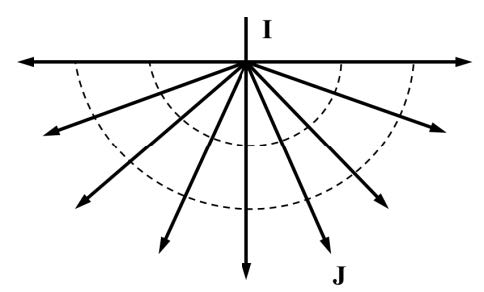
\includegraphics[width=0.4\textwidth]{1.jpg}
                \caption{电流 $I$ 以点接触的形式注入到半无穷大样品内部的电流密度分布}
            \end{figure}
        \subsubsection{无穷大薄样品体电阻率的测量}
            类似前面的分析,无穷大薄样品的体电阻率 $\rho$ 可表示为:
            \begin{equation}
                \rho =\frac{\pi V_{23}}{I \ln 2} \label{eq:1}
            \end{equation}
    \subsection{半导体材料电阻的测量}        
        \subsubsection{半导体薄层电阻(或方块电阻)的测量}
            如果扩散片的结深用 $X_j$ 表示,根据定义,方块电阻 $R_{sq}$ 可表示为:
            \begin{equation}
                R_{sq}=\rho\frac{L}{L\cdot X_{j}}=\frac{\rho}{X_{j}} \label{eq:2}
            \end{equation}
            将 \seqref{eq:1} 代入 \seqref{eq:2} 得:
            \begin{equation}
                R_{sq}=4.5324\frac{V_{23} d}{I} \label{eq:3}
            \end{equation}
            实际测量中,只要薄层的厚度小于 $0.5S$,并且样品面积相对于探针间距 $S$ 可视为无穷大时,就可以利用\seqref{eq:3}计算薄层电阻。如果不能将样品的横向面积视为无穷大,也需要使用包含修正因子 $F$ 的公式来计算方块电阻:
            \begin{equation}
                R_{sq}= F \frac{V_{23}}{I} \label{eq:4}
            \end{equation}
        
\section{实验仪器}%规格及参数
    KDY-1 型四探针电阻率/方阻测试仪,一台计算机;p 型单晶硅棒(电阻率样品)、p 型单晶硅片(薄样品)、p 型硅基底上的 n 型扩散片(薄层电阻样品)各一个
\section{实验过程}%简述主要过程和实验内容
    \subsection{测量样品电阻率或方块电阻的操作步骤}
    \begin{enumerate}
        \item 打开 KDB-1 四探针测试仪后面板上的电源开关,此时恒流源已开启,测试电流自动处于 \SI{1}{\milli\ampere} 档。根据测试目的,将测试仪后面板上的 “电阻率/方块电阻测试切换开关”($\rho/R$ 开关)拨到相应位置。
        \item 将样品置于样品台上,旋转测试架上的手轮使探针下降,同时调整样品位置,使四根探针正好落在样品的测试点。当探针快要接触样品时,应缓慢旋转手轮,使探针缓慢轻压在样品上。当听到主机传来“咔嗒”一声、且前面板左侧的两块绿字电表有数值显示,即表示探针与样品已接触到位,应立即停止旋转手轮。
        \item 根据附表给出的推荐值,并通过选择合适的测试电流档位和恒流源电压档位,调节测试电流和恒流源电压旋钮,使测试电流达到合适的值,此时,电压表显示的 $V_{23}$ 应出现尽可能多的有效数字,且电压值在测试电流不变的前提下能长时间保持稳定,而且正测和反测得到的 $V_{23}$ 的绝对值差别也不大。
        \item 记录此时的测试电流 I 和电压 $V_{23}$ 的值,由相应公式计算样品的电阻率或方块电阻。测量完毕,升起探针,取走样品。
    \end{enumerate}
    \subsection{测量 p 型硅棒的电阻率}
        使用厂家推荐的测试电流对硅棒横截面上五个不同位置处(中心点和距离圆心 1/3 半径处的 4 个等距点)的电阻率进行测量。为了减小测量误差,对同一点的测量分别进行正向和反向测量。将实验结果记录到表中,使用\seqref{eq:0} 计算电阻率 $\rho (T)$。利用附录将测得的电阻率修正到 \SI{23}{\degreeCelsius}。此外,利用下面的公式计算电阻率分布的不均匀度。
    \subsection{测量 p 型单晶硅片(薄样品)的电阻率}
        \begin{enumerate}
            \item 直读法,根据样品厚度和附表 4 得到直读电流的值,并将其设置为测试电流,直接
            从电压表上读取样品的电阻率。
            \item 选择合适的测试电流 I 和测得的电压 $V_{23}$,采用 $\rho(T)=\frac{V_{23}}l\cdot d\cdot F_{SP}\cdot F(d/S)\cdot F(S/D)$ 计算硅片的电阻率。对硅片中心位置处的电阻率测量 5 次。每次测量完毕后,升起探针,将硅片逆时针旋转 $\SI{30}{\degree} \sim  \SI{35}{\degree}$ 进行下一次测量。同一位置正向和反向各测量一次,并将测量结果修正到 \SI{23}{\degreeCelsius}。
        \end{enumerate}
    \subsection{测量 p 型单晶硅衬底上的 n 型扩散片的方块电阻 }
        扩散片的结深 $X_j$ 和尺寸由老师现场提供。由于待测扩散片近似正方形,故取最短的边长作为扩散片的直径 $D$ 。将探针压在扩散片的中心位置进行方块电阻的测量。
        \begin{enumerate}
            \item 直读法,设置合适的测试电流,从电压表上直接读出样品的方块电阻。
            \item 根据测试电流、电压 $V_{23}$ 以及扩散片的尺寸,利用\seqref{eq:4}计算扩散片的方块电阻。需要测量两个位置的方块电阻,即在第一次测量完成之后将样品旋转 \SI{90}{\degree} 再测量一次。同一位置正向和反向各测量一次。
        \end{enumerate}
    \subsection{测量 p 型单晶硅衬底上的 n 型扩散片的方块电阻 }
        本实验提供两种透明导电玻璃(FTO 导电玻璃和 ITO 玻璃),测试方法及要求与测试扩散片一致。
\end{document}